\chapter{Architettura del sistema}
\label{ch:architettura}

In questa sezione verranno descritte a livello funzionale le varie componenti del sistema e classificate secondo il modello visto a lezione.

In figura~\ref{fig:architettura} è riportata una vista architetturale ad alto livello del sistema. La figura non riporta le interfacce di \textit{callback} per non renderne difficile la fruizione. La parte riguardante l'invio di messaggi dalla componente \evdisp{} verso il resto del sistema viene infatti trattata in dettaglio nella sezione~\ref{sec:dispatcherImpl}, mentre l'uso di \textit{callback} da parte di \sched{} viene discusso in~\ref{sec:scheduler}. Vengono inoltre omesse dal diagramma le componenti che si occupano dell'inizializzazione del prototipo, descritte invece in dettaglio nella sezione~\ref{sec:start-stop}.

\begin{landscape}
\begin{figure}
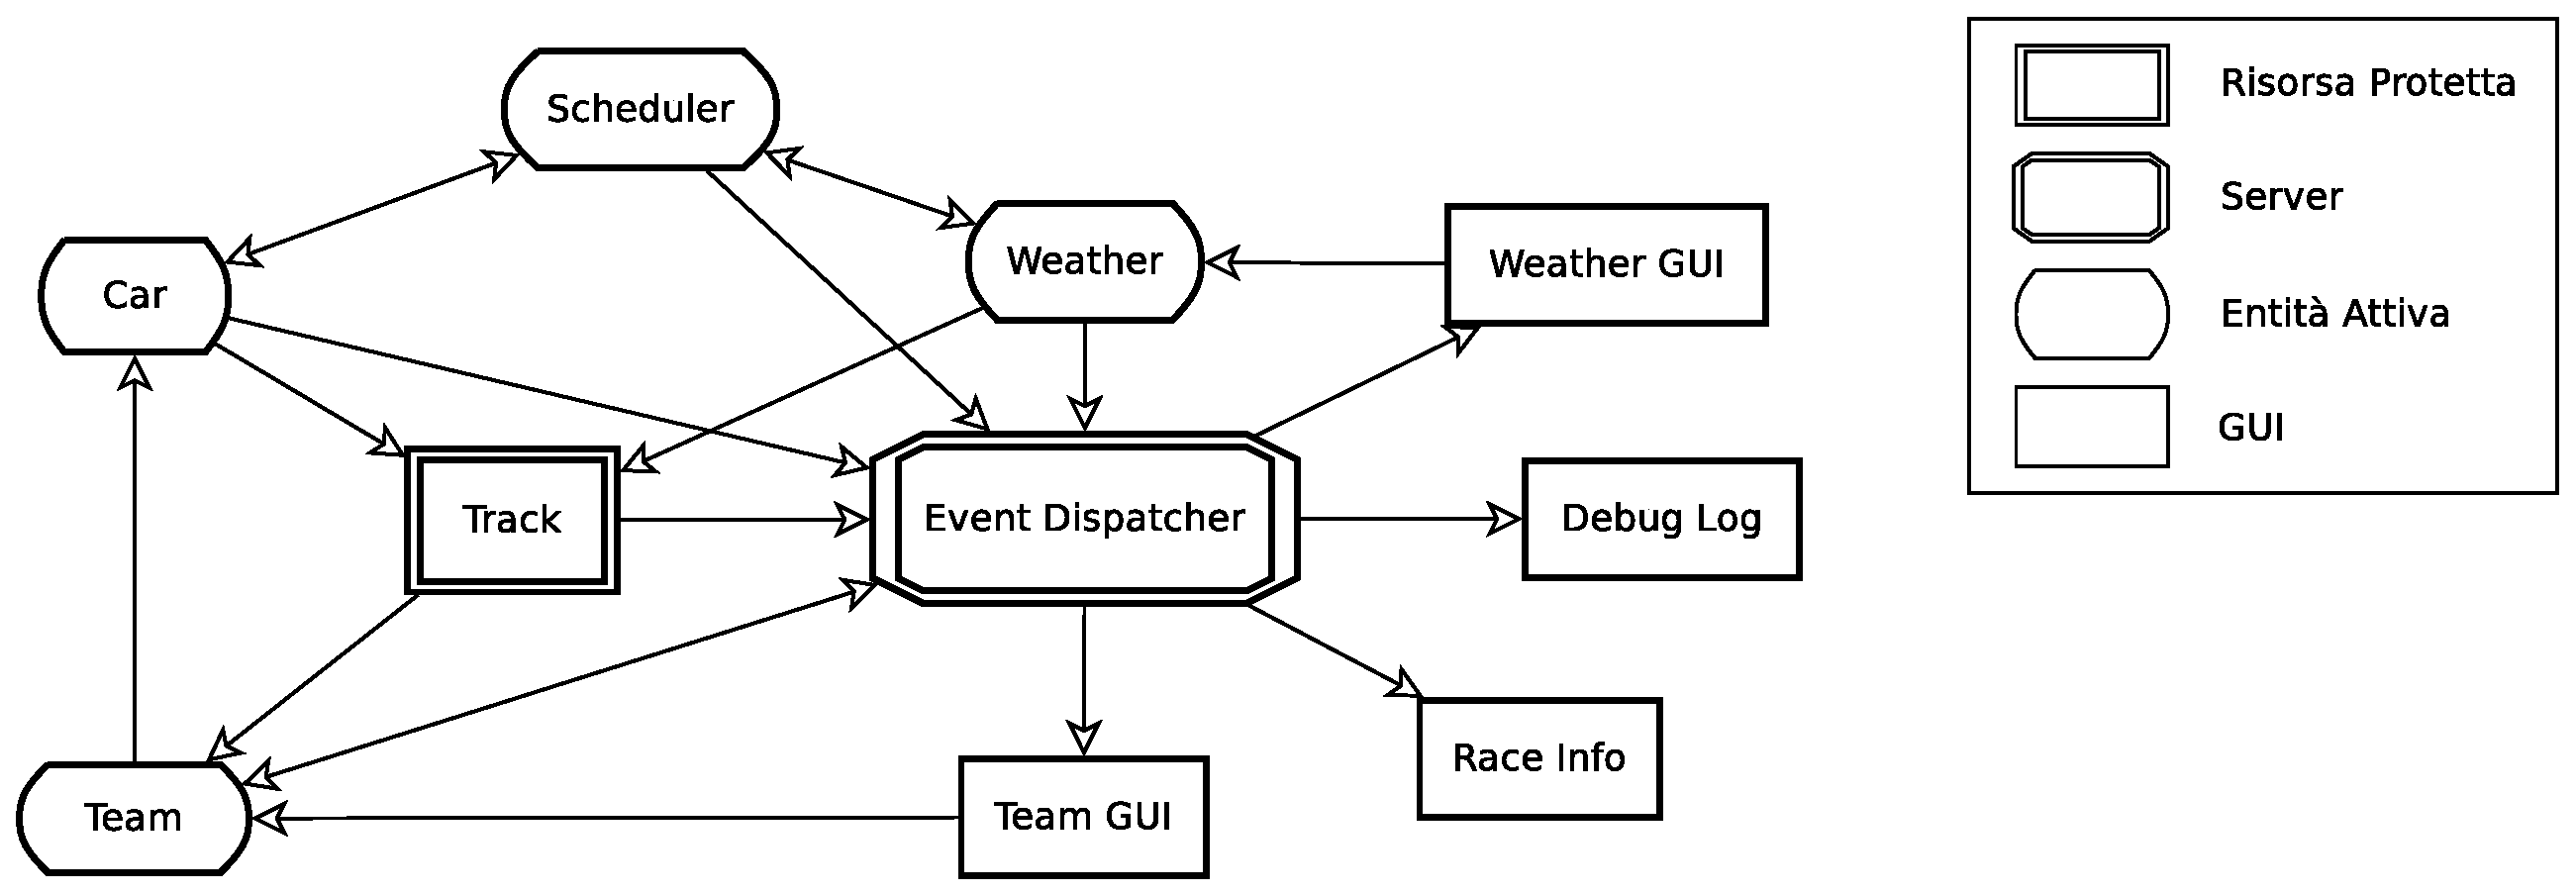
\includegraphics[height=.42\paperheight]{diagrammi/Arch}
\caption{Architettura di sistema}
\label{fig:architettura}
\end{figure}
\end{landscape}

\section{Event Dispatcher}
\label{sec:dispatcherArch}
Questa componente ha il compito di ricevere tutti i dati relativi alla competizione e, dopo una eventuale rielaborazione, inoltrare tali dati alle componenti interessate.

Questo tipo di comunicazione segue il \textit{pattern} architetturale \textit{\mbox{publish/subscribe}} ed è quindi previsto che le componenti del sistema interessate a tali dati effettuino prima la procedura di \textit{subscription} (ricevendo se necessario lo stato attuale della gara) per poi ottenere aggiornamenti con l'evolvere della simulazione. Gli aggiornamenti vengono inviati dalla componente \evdisp{} ai \textit{subscribers}, con uno stile di comunicazione di tipo \textit{push}, come d'altronde previsto dal \textit{pattern} adottato.

I \textit{subscribers} devono indicare che informazioni desiderano ricevere di modo che \evdisp{} possa effettuare una procedura di filtraggio per evitare l'invio di dati non richiesti.

\evdisp{} assume quindi il ruolo di \textit{message broker} poiché smista e traduce i messaggi provenienti dai \textit{publishers} e li inoltra ai \textit{subscribers}. In questo modo si ottiene un basso livello di accoppiamento, a dimostrazione di ciò è sufficiente notare che non è nemmeno necessario che il gruppo delle componenti \textit{publishers} sia al corrente dell'esistenza delle componenti \textit{subscribers}.

\`E previsto inoltre che un \textit{subscriber} possa registrarsi presso \evdisp{} in un qualsiasi momento dopo la fase di \textit{bootstrap} e prima della terminazione della simulazione. Per questo motivo \evdisp{} deve essere progettato per fornire informazioni coerenti anche ai \textit{subscribers} che si aggiungono al sistema a simulazione iniziata.

Viste le caratteristiche che deve avere tale componente, nell'ottica di un sistema distribuito possiamo considerarla un server poiché non effettua comunicazioni con altre componenti del sistema se non in risposta ad azioni esterne, rientrando quindi nella categoria delle entità reattive.

\subsection*{Interfaccia fornita}
\evdisp{} deve fornire metodi di interfaccia verso due insiemi di attori:
\begin{itemize}
\item \textit{subscribers}, ovvero i processi che si registrano per ottenere le informazioni riguardanti la gara attraverso il metodo \fun{subscribe},
\item \textit{publishers}, ovvero quei processi che scatenano eventi inerenti la competizione e delegano la notifica al sistema di tali eventi ad \evdisp{} tramite l'invocazione del metodo \fun{notify}.
\end{itemize}
Il metodo \fun{subscribe} prevede che il processo chiamante indichi tra i parametri anche una funzione di \textit{callback} che faccia da canale per l'invio delle notifiche di gara.

\subsection*{Interfaccia richiesta}
Da un punto di vista puramente pratico non vi è nessuna interfaccia richiesta da questa componente poiché \evdisp{}, in assenza di \textit{subscribers}, non effettua invocazioni di metodi. Tuttavia abbiamo preferito considerare l'interfaccia richiesta come dinamica, ovvero inizialmente vuota e che acquisisce metodi all'aumentare del numero di \textit{subscribers}. Al momento della registrazione i \textit{subscribers} devono indicare ad \evdisp{} quale metodo di \textit{callback} utilizzare e che va quindi ad aggiungersi all'interfaccia richiesta della presente componente.


\section{Scheduler}
\label{sec:scheduler}
La componente \sched{} ha lo scopo di definire e gestire l'ordine di esecuzione dei processi quando essi devono accedere alla componente \track{}.
Le entità arbitrate sono i processi \car{}, che simulano gli spostamenti delle auto durante la gara, e il processo \weather{}, che gestisce le variazioni alle condizioni meteo del tracciato.

L'idea di base di questa componente è di mantenere un orologio ``logico'' unico relativo alla competizione e di permettere l'esecuzione dei soli processi che si sono precedentemente prenotati. Si tratta perciò di un sistema di \textit{booking} nel quale i processi che vengono serviti devono prima indicare a che tempo di gara vogliono eseguire e successivamente vengono messi in una coda ordinata secondo il tempo indicato nella prenotazione. Tra tutti i processi accodati lo \sched{} eleggerà per l'esecuzione sempre quello in testa, ovvero il processo che nella fase di prenotazione precedente ha indicato un tempo di gara minore. Questa componente ha quindi la funzione di eliminare la parte indesiderata di concorrenza presente nel sistema, per rendere predicibile e controllata l'evoluzione della simulazione.

Al momento della prenotazione, \car{} e \weather{} devono indicare anche un metodo di \textit{callback}. L'invocazione di tale metodo da parte dello \sched{} equivale al permesso di eseguire e quindi accedere a \track{}, come richiesto nella fase di prenotazione.
L'invocazione di \textit{callback} è effettuata con una chiamata bloccante in modo da permettere a \sched{} di conoscere quando il processo richiedente ha terminato di utilizzare la risorsa \track{}.

L'uso di \textit{callbacks} rende omogenea la trattazione dei diversi processi, riducendo notevolmente l'accoppiamento.

Per poter soddisfare le caratteristiche sopra indicate è risultato naturale progettare l'entità \sched{} come attiva.

\subsection*{Interfaccia fornita}
Lo \sched{} deve fornire un metodo \fun{queue\_work} che permette alle altre entità attive di effettuare la procedura di \textit{booking} precedentemente descritta.
Il metodo \fun{set\_speedup} serve a regolare la velocità con cui evolve la simulazione, mentre i metodi \fun{start\_simulation} e \fun{pause\_simulation} servono rispettivamente ad avviare e fermare momentaneamente la simulazione.

\subsection*{Interfaccia richiesta}
Nessuna.

\section{Track}
La componente \track{} è stata pensata per incapsulare i dati relativi al circuito di gara e le regole di percorrenza del medesimo. Dal punto di vista progettuale \track{} è sicuramente un'entità reattiva, in particolare una risorsa protetta con agente di controllo passivo.
I dati relativi alla configurazione della pista utilizzati dal sistema sono derivati dalle informazioni inserite dall'utente tramite file di configurazione.

La componente \track{} deve contenere due gruppi di dati, uno riguardo le informazioni che possono essere considerate costanti poiché non variano nell'arco della competizione, l'altro comprendente i dati dinamici come la posizione delle vetture durante la gara.
La rappresentazione interna della pista è gestita come una lista di segmenti ciascuno dei quali contiene le seguenti informazioni:
\begin{itemize}
\item lunghezza del tratto,
\item indice minimo di corsia,
\item indice massimo di corsia,
\item inclinazione,
\item raggio di curvatura (nel caso in cui il segmento sia una curva).
\end{itemize}
Associate ai segmenti si hanno informazioni dinamiche riguardanti lo stato della pista come le condizioni atmosferiche al suolo.
Un altro gruppo di informazioni dinamiche fondamentali contenute in \track{} è quello relativo alle auto, per ogni auto infatti sono presenti:
\begin{itemize}
\item segmento che sta percorrendo,
\item tempo e corsia di ingresso nel segmento,
\item tempo e corsia di uscita dal segmento,
\item velocità di uscita dal segmento.
\end{itemize}

Oltre ai dati visti finora, la componente \track{} deve anche gestire la logica che determina quali spostamenti siano concessi alle auto e soprattutto secondo quali vincoli tali spostamenti siano possibili. Deve quindi esporre un metodo che permetta alle auto di simulare l'esito di un eventuale spostamento nella pista e un metodo che invece implementi l'effettivo spostamento dell'auto. Fornire un metodo per la simulazione della mossa permette di dare dei dati al chiamante che può quindi scegliere, secondo la sua logica interna e strategia di gara, quale sia la migliore mossa da eseguire e in un momento successivo effettuare tale mossa.

\subsection*{Interfaccia fornita}
Grazie al metodo \fun{simulate} le entità \car{} possono simulare l'esito di uno spostamento, una volta scelta la corsia di uscita ed espressa la volontà o meno di effettuare una sosta ai \textit{box} in quel giro.

La presenza del metodo \fun{simulate} è giustificata dal fatto che la logica di \car{}, al fine di scegliere il modo migliore di percorrere un segmento, ha bisogno non solo di informazioni sulla fisica dello stesso ma deve considerare anche l'interazione che l'auto può avere con altre eventuali vetture che stanno percorrendo il medesimo segmento.

Grazie a questo metodo \car{} può conoscere i tempi di percorrenza del segmento (uno per ogni corsia raggiungibile dall'auto) prima di effettuare l'effettivo spostamento sulla pista e scegliere conseguentemente la corsia di uscita ritenuta migliore.

Il metodo \fun{move} necessita degli stessi parametri del metodo \fun{simulate} e serve a spostare effettivamente l'auto sul tracciato di gara e ad effettuare le eventuali notifiche di eventi scatenati da tale spostamento.

\subsection*{Interfaccia richiesta}
Da un punto di vista funzionale la componente \track{} contiene il meccanismo che guida l'erogazione delle operazioni di rifornimento, tuttavia non può decidere quali operazioni effettuare, poiché questo tipo di scelte è inerente la strategia di gara e quindi è da considerarsi a carico della componente \team{}. Di conseguenza \track{} necessita di un metodo \fun{pitstop\_operations} da invocare presso la componente \team{} associata all'auto ai \textit{box}, tale metodo deve avere come valore di ritorno le informazioni su che operazioni di rifornimento da effettuare.

Durante la simulazione, nel momento in cui un'auto effettua uno spostamento, è la componente \track{} che riconosce eventi come un sorpasso o l'attraversamento di un intermedio cronometrico e deve provvedere ad inviare le notifiche di tali eventi al sistema. La componente \track{} non deve tuttavia incaricarsi di notificare direttamente tali eventi a chi è interessato ma, come previsto dall'architettura di sistema, si limita ad inviare le notifiche alla componente \evdisp{} e delega a quest'ultima la propagazione di tali informazioni nel sistema.
Le notifiche possibili riguardano:
\begin{itemize}
\item sosta ai \textit{box} ed operazioni effettuate,
\item ritiro dalla gara di un'auto,
\item attraversamento di un intermedio cronometrico,
\item sorpasso,
\item fine della gara.
\end{itemize}

\section{Car}
\car{} è un'entità attiva e rappresenta nel contesto del progetto un'auto che partecipa alla competizione. Ad ogni istanza di questa componente presente nel sistema saranno associate le seguenti informazioni:
\begin{itemize}
\item numero identificativo,
\item nome del pilota,
\item abilità del pilota,
\item peso del pilota,
\item scuderia di appartenenza,
\item livello di carburante nell'auto,
\item tipo di pneumatici utilizzati,
\item livello di usura dei pneumatici.
\end{itemize}
Prima dell'inizio della competizione \car{} deve prenotarsi presso lo \sched{} e stare poi in attesa del permesso di muoversi sulla pista.
Questa componente ha il compito di decidere quale traiettoria adottare per percorrere un segmento e deve farlo basandosi sullo stato dell'auto, sulle direttive dei \team{} e dell'utente e sulle informazioni fornite da \track{}.

\subsection*{Interfaccia fornita}
L'autorizzazione a muoversi sul circuito di gara viene data a questa componente dallo \sched{} attraverso l'invocazione del metodo \fun{move}. L'esecuzione di questo metodo è divisa in due fasi:
\begin{itemize}
\item simulazione, ovvero la fase in cui \car{} utilizza l'interfaccia fornita dalla componente \track{} per simulare tutte le mosse consentite e decidere, secondo la logica che governa la strategia di gara del pilota, quale tra le possibili traiettorie adottare.
\item spostamento, consiste nel segnalare a \track{} la mossa decisa dall'auto e, a fronte delle conseguenze che tale spostamento comporta, prenotarsi nuovamente presso lo \sched{} nel caso in cui la mossa vada a buon fine, ritirarsi altrimenti.
\end{itemize}

Per permettere la comunicazione della strategia di gara tra \team{} e \car{}, la presente componente deve esporre nella sua interfaccia un metodo \fun{set\_next\_pitstop} che serve alla scuderia per comunicare al pilota in quale giro recarsi ai \textit{box} per il rifornimento.

L'utente può anche decidere di forzare il pilota ad effettuare mosse non previste dalla strategia di gara e che non possono essere modificate se non dall'utente stesso, in particolare può:
\begin{itemize}
\item imporre una sosta ai \textit{box} il prima possibile, per questo viene fornito il metodo \fun{force\_pitstop},
\item forzare il ritiro dalla competizione, a tale scopo viene esposto dall'interfaccia il metodo \fun{retire}.
\end{itemize}

\subsection*{Interfaccia richiesta}
Questa componente necessita delle funzionalità \fun{simulate} (fase di simulazione) e \fun{move} (fase di spostamento) fornite dalla componente \track{} per poter realizzare il metodo \fun{move} prima descritto.
Durante la fase di inizializzazione del sistema ogni componente \car{} deve notificare i dati di interesse relativi alla sua configurazione al resto del sistema. Questo viene ottenuto grazie al canale \fun{notify} fornito da \evdisp{}.

\section{Team}
Questa componente nel contesto della simulazione rappresenta le scuderie in gara. \team{} deve quindi ricevere i dati relativi alle prestazioni delle proprie auto e allo stato della pista, elaborare una strategia di rifornimento e comunicare alle auto quando recarsi ai \textit{box}.

Le decisioni che la logica di questa componente deve prendere sono inerenti le operazioni da eseguire in fase di rifornimento e comprendono la quantità di carburante aggiuntivo da imbarcare, se sostituire o meno i pneumatici ed eventualmente il tipo di pneumatici più appropriato alle condizioni atmosferiche della pista.

\subsection*{Interfaccia fornita}
\team{} espone il metodo \fun{pitstop\_operations} nella sua interfaccia con lo scopo di fornire alla componente \track{}, durante la fase di sosta ai \textit{box} di un'auto, le informazioni necessarie ad effettuare le operazioni di rifornimento.

Il metodo \fun{update} fornisce un canale di comunicazione che \evdisp{} usa per la notifica di eventi relativi alla gara considerati importanti per le scuderie.

\subsection*{Interfaccia richiesta}
Per poter comunicare la strategia di gara decisa alle auto appartenenti alla scuderia rappresentata, questa componente necessita del metodo \fun{set\_next\_pitstop} fornito da \car{}.
Come la componente \car{} anche \team{} deve comunicare le proprie informazioni di configurazione al sistema tramite il metodo \fun{notify} di \evdisp{}.

\section{Weather}
\weather{} è la componente del sistema addetta a gestire le condizioni meteorologiche iniziali sulla pista e le variazioni di tali condizioni durante la competizione. Tali variazioni sono decise dall'utente tramite file di configurazione, oppure possono essere decise a simulazione avviata in modo asincrono tramite interfaccia utente.

Poiché questa entità attiva va a modificare lo stato della pista, essa è evidentemente in concorrenza con le entità \car{} presenti nel sistema. \`E pertanto necessario che l'accesso alla risorsa \track{} avvenga in modo controllato: in particolare è previsto che le modifiche sulla pista avvengano attraverso \textit{booking} presso lo \sched{}.

\subsection*{Interfaccia fornita}
Al momento della prenotazione presso lo \sched{} questa componente indica il metodo \fun{apply\_change} come metodo di \textit{callback}. Così facendo l'accoppiamento tra le due componenti è mantenuto minimo. Questo metodo ha il compito di cambiare il tempo atmosferico di \track{} secondo quanto precedentemente definito dall'utente.

L'altro metodo che l'interfaccia di \weather{} espone è \fun{schedule\_change} che serve per impostare eventuali ulteriori variazioni a simulazione avviata.

\subsection*{Interfaccia richiesta}
Conformemente a quanto visto finora, anche la modifica del tempo atmosferico necessita dell'autorizzazione dello \sched{} per essere portata a termine poiché richiede l'accesso a \track{}. Di conseguenza tutte le modifiche saranno procedute da un'invocazione del metodo \fun{queue\_work} dello \sched{} per assolvere alla fase di prenotazione.

Le condizioni atmosferiche sono un fattore importante per la simulazione e una variazione delle medesime può essere di interesse a diverse componenti del sistema. Per questo motivo ogni volta che viene invocato il metodo \fun{apply\_change}, viene notificata la modifica grazie al metodo \fun{notify} di \evdisp{}.

\section{Debug Log}
Questa componente è pensata principalmente per essere d'ausilio nella fase di sviluppo e test rendendo disponibili i dati in formato testuale tramite una semplice interfaccia grafica.

In fase di inizializzazione essa effettua la procedura di \textit{subscription} presso \evdisp{}, assumendo quindi il ruolo di \textit{subscriber} nel \textit{pattern} descritto in~\ref{sec:dispatcherArch}.

\subsection*{Interfaccia fornita}
Al fine di poter riceve le notifiche da \evdisp{} questa componente espone in interfaccia un metodo di \textit{callback} che serve a ricevere le notifiche e mostrare le informazioni trasportate in forma testuale all'utente.

\subsection*{Interfaccia richiesta}
Facendo parte del gruppo di componenti \textit{subscribers}, \texttt{debug\_log} necessita della possibilità di registrarsi presso \evdisp{} con il metodo \fun{subscribe}.

\section{Race Info}
Questa componente raggruppa la maggior parte delle funzionalità di visualizzazione della competizione e permette inoltre all'utente di interagire con il sistema.

I dati visualizzati devono essere sufficienti all'utente per comprendere l'andamento della gara. Devono quindi essere presenti:
\begin{itemize}
\item stato della simulazione (avviata, in pausa, terminata),
\item posizione delle auto sulla pista,
\item classifica e sorpassi,
\item eventuali ritiri,
\item velocità massima,
\item tempo migliore sul giro.
\end{itemize}
Attraverso questa componente l'utente può interagire con lo stato della simulazione nei seguenti modi:
\begin{itemize}
\item avvio,
\item pausa,
\item modifica del fattore di \textit{simulation speed}.
\end{itemize}

\subsection*{Interfaccia fornita}
Essendo \texttt{race\_info} una GUI, dal punto di vista funzionale espone sicuramente un'interfaccia verso l'utente con lo scopo di rendere facilmente fruibili i dati riguardanti l'evolvere della simulazione.
Questa componente ricopre il ruolo di \textit{subscriber}, come descritto in~\ref{sec:dispatcherArch}, e riceve quindi le informazioni sulla competizione da \evdisp{}. Per questo motivo, in accordo con il \textit{pattern} architetturale usato, deve fornire ad \evdisp{} almeno un canale di comunicazione (metodo di \textit{callback}).

\subsection*{Interfaccia richiesta}
Per poter interagire con la simulazione come descritto precedentemente \texttt{race\_info} necessita di diversi metodi forniti della componente \sched{}:
\begin{itemize}
\item \fun{start\_simulation},
\item \fun{pause\_simulation},
\item \fun{set\_speedup}.
\end{itemize}
Appartenendo inoltre al gruppo dei \textit{subscribers} questa componente necessita del metodo \fun{event\_dispatcher:subscribe}.

\section{Team Monitor}
Questa componente è un'interfaccia grafica che serve a fornire all'utente dettagli approfonditi sulle statistiche di gara delle auto appartenenti ad una determinata scuderia.
I dati da mostrare all'utente sono:
\begin{itemize}
\item nome del pilota,
\item carburante residuo,
\item tipo e stato dei pneumatici,
\item tempo migliore per intermedio cronometrico,
\item tempo migliore sul giro,
\item tempi realizzati nell'ultimo giro,
\item velocità massima raggiunta in ciascun intermedio cronometrico,
\item numero di \textit{pit stop} effettuati,
\item operazioni effettuate durante l'ultima sosta ai \textit{box}.
\end{itemize}
L'utente può inoltre forzare la sosta ai \textit{box} o il ritiro per un'auto appartenente alla scuderia.

Questa componente ricopre il ruolo di \textit{subscriber}, come descritto in~\ref{sec:dispatcherArch}.

\subsection*{Interfaccia fornita}
Le informazioni sulla gara sono ottenute tramite \evdisp{}, di conseguenza, \texttt{team\_monitor} deve esporre i canali di comunicazione necessari come metodi di \textit{callback}.
\subsection*{Interfaccia richiesta}
Al fine di permettere all'utente l'interazione con le auto appartenenti alla scuderia, questa componente necessita dei metodi \fun{retire} e \fun{force\_pitstop} esposti da \car{}.

Per poter registrarsi presso \evdisp{}, ed ottenere quindi le informazioni da mostrare all'utente, \texttt{team\_monitor} necessita del metodo \\\fun{event\_dispatcher:subscribe}.

\section{Weather Station}
Questa componente è un'interfaccia grafica che mostra all'utente le condizioni atmosferiche sulla pista e permette ad esso di modificarle durante il corso della competizione. Le informazioni sullo stato della pista sono ottenute tramite notifiche da \evdisp{} mentre le richieste di variazioni vengono inviate alla componente \weather{}.
Questa componente ricopre il ruolo di \textit{subscriber}, come descritto in~\ref{sec:dispatcherArch}.

\subsection*{Interfaccia fornita}
Deve fornire un \textit{callback} per la ricezione dei dati inerenti le condizioni atmosferiche sul circuito di gara.
\subsection*{Interfaccia richiesta}
Essendo questa una componente \textit{subscriber}, essa richiede le funzionalità offerte da \fun{event\_dispatcher:subscribe}.

Per quanto riguarda invece la modifica delle condizioni atmosferiche è necessario che la componente \weather{} esponga in interfaccia il metodo \fun{schedule\_change}, in modo da permettere a \texttt{weather\_station} di comunicare le variazioni decise dall'utente a simulazione avviata.

\section{Avvio e terminazione}
\label{sec:start-stop}
Per rendere più usabile il prototipo abbiamo pensato di far svolgere l'avvio e la configurazione del sistema tramite interfaccia grafica.
L'utente dovrà interagire con due tipi di interfacce di configurazione:
\begin{itemize}
\item \texttt{control\_panel}: permette all'utente di inserire il percorso dei file di configurazione, nonché di per avviare e terminare il sistema.
\item \texttt{node\_configurator}: serve all'utente per indicare al sistema su quali nodi possono essere avviate le componenti essenziali del sistema e per determinare quindi come saranno distribuite sulla rete tali componenti.
\end{itemize}

Per gestire l'avvio e la terminazione del sistema in modo indipendente dalla distribuzione delle componenti di simulazione abbiamo deciso di associare ad ogni nodo che partecipa al sistema un processo per il controllo del nodo stesso. Vi sarà quindi un nodo controllato da \bootserv{} che non partecipa alla simulazione e un numero variabile di nodi gestiti da altrettanti \nodeman{} sui quali vengono eseguite le componenti di simulazione. Questi processi di controllo non devono terminare finché il nodo serve al sistema poiché hanno il compito fondamentale di terminare il nodo stesso alla chiusura del sistema.

\subsection{Control Panel e Bootstrap Server}
\texttt{control\_panel} ha il compito di acquisire le informazioni necessarie alla simulazione dall'utente e avviare la componente \bootserv{}. Dopodiché \texttt{control\_panel} deve rimanere attivo poiché è l'interfaccia che permette all'utente di terminare tutti i nodi del sistema.

La funzione di \bootserv{} è fondamentale per l'avvio e la terminazione del sistema e di conseguenza non deve essere terminato finché gli altri nodi del sistema sono attivi.

Nella fase iniziale il suo compito è quello di coordinare l'inizializzazione di tutte le componenti del sistema nell'ordine corretto, secondo la disponibilità dei nodi e le necessità della simulazione, rispettando le dipendenze di avvio tra le varie entità.
Il numero di componenti da istanziare viene calcolato come segue: per quanto riguarda \car{} e \team{}, i requisiti minimi vengono ricavati in modo automatico a partire dai file di configurazione, mentre è comunque sempre necessaria un'istanza per ciascuna delle componenti: \evdisp{}, \sched{}, \weather{}. Finché il sistema non è formato da un numero di nodi con una disponibilità di risorse sufficiente ad ospitare la simulazione, esso non può essere avviato.

Una volta che \bootserv{} ha istanziato nel giusto ordine le componenti necessarie presso i nodi distribuiti, la fase di \textit{bootstrap} del sistema può dirsi conclusa.
Successivamente \bootserv{} rimane in attesa del comando di terminazione da parte di \texttt{control\_panel} per coordinare la terminazione dei nodi del sistema distribuiti.

\subsection{Node Configurator e Node Manager}
Una volta avviato, \texttt{node\_configurator} istanzia un nodo che andrà a fare parte del sistema distribuito e ivi avvia \nodeman{}. L'utente deve indicare tramite l'interfaccia grafica \texttt{node\_configurator} la disponibilità di risorse del nodo appena avviato in modo che \nodeman{} possa comunicarlo a \bootserv{}.

La componente \nodeman{} ha anche il compito di avviare le componenti necessarie alla simulazione indicategli e su delega del \bootserv{}.

Una volta terminata la fase di \textit{bootstrap} del sistema, \nodeman{} deve rimanere in attesa del comando di terminazione del nodo che verrà eventualmente inviato da \bootserv{}, mentre \texttt{node\_configurator} viene terminato una volta che l'utente ha inserito le informazioni necessarie.

\subsection{Terminazione}
\`E opportuno distinguere tra terminazione della simulazione e terminazione del sistema.
La terminazione della simulazione comporta la terminazione dei processi \sched{}, \evdisp{}, \team{}, \car{} e \weather{}, in ordine inverso rispetto a quello di avvio, oltre alla deallocazione dei dati riguardanti la pista e dei parametri di configurazione della competizione. Le interfacce grafiche sono informate della terminazione tramite un'opportuna notifica, ma non vengono chiuse automaticamente perché l'utente potrebbe necessitare di tempo ulteriore per analizzare i dati da esse visualizzati.

La terminazione del sistema, invece, coinvolge anche la terminazione delle componenti:
\begin{itemize}
\item \bootserv{}
\item \nodeman{}
\item \texttt{control\_panel}
\end{itemize}
Infine vengono terminati tutti i nodi del sistema.

Dividendo in questo modo la fase di terminazione è possibile effettuare più simulazioni senza dover riavviare il sistema ma semplicemente terminando la simulazione corrente e riconfigurandone una di nuova tramite \texttt{control\_panel}. \`E quindi possibile riutilizzare i nodi già avviati e ridurre il numero di componenti istanziate \textit{ex novo} al minimo necessario.
